\documentclass{article}
% bibliography setup
\usepackage{natbib}
\bibliographystyle{apalike}  % abbrvnat
\setcitestyle{authoryear,open={(},close={)}} %Citation-related commands
% makes color citations
\usepackage[colorlinks=true,urlcolor=blue,citecolor=red,linkcolor=red,bookmarks=true]{hyperref}
% images
\usepackage{graphicx}
\graphicspath{ {./images/} }

% hypter parameter setup
\usepackage{hyperref}


\title{Improved Sequential Hypothesis Testing with
``Enhanced Precision Is The Goal"}
\date{\today}
\author{Eyal A. Kazin}

\begin{document}
\maketitle

\input precision_goal_abstract

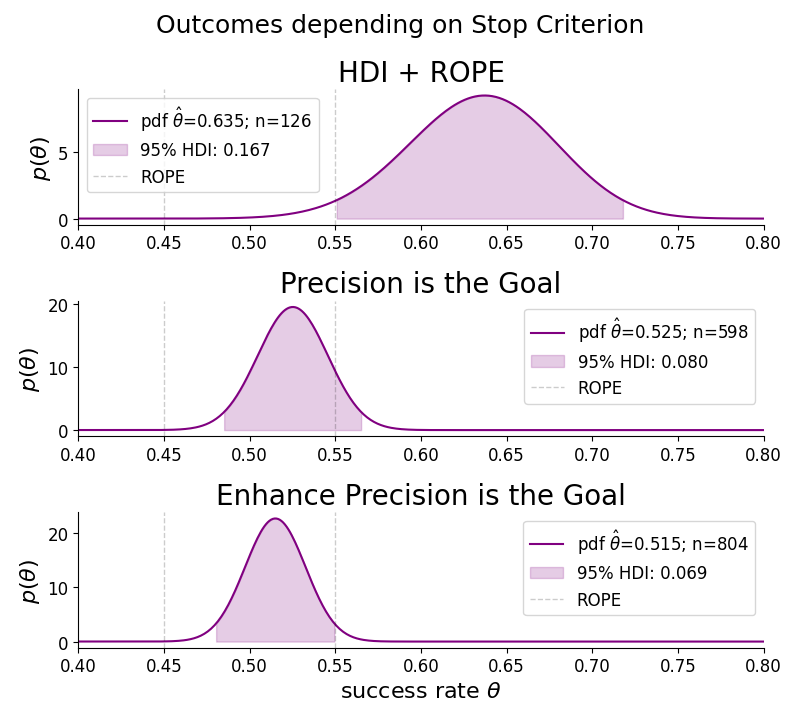
\includegraphics[scale=0.5]{cherry_posteriors.png}

%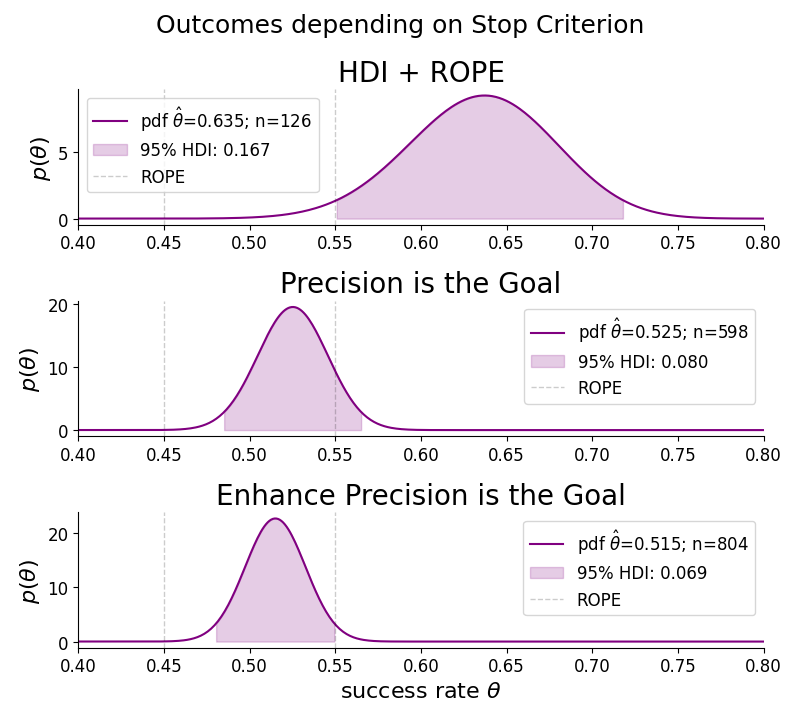
\includegraphics[width=1\textwidth]{cherry_posteriors.png}

\begin{figure}[h]
    \centering
    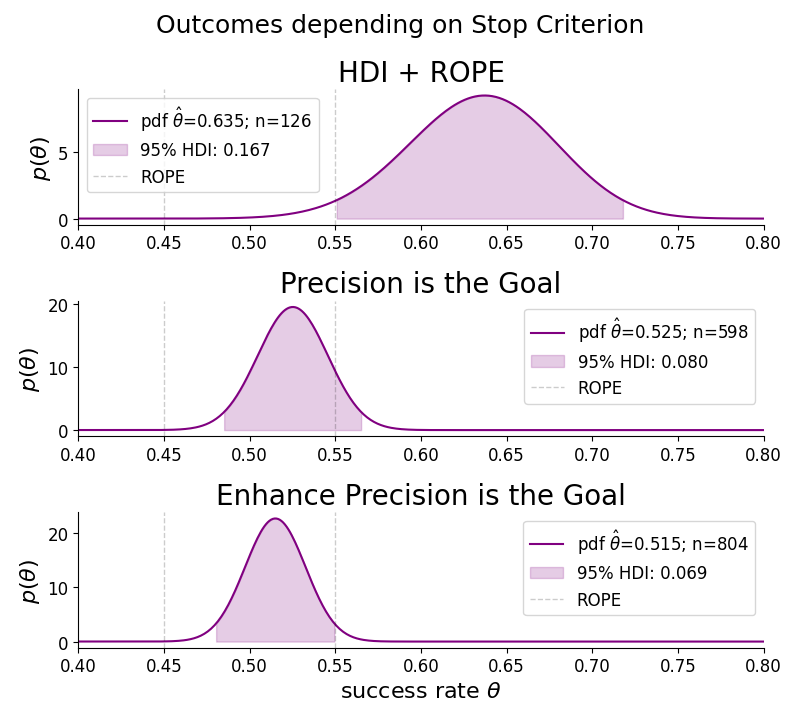
\includegraphics[width=1\textwidth]{cherry_posteriors.png}
    \caption{Beta function posteriors of subsamples of example sequence from Figure REF. Panels are results of different stop/decision criteria being triggered. Shaded areas are 95\% HDIs. ROPE within vertical dashed lines.
    Top - HDI+ ROPE triggers when the 95\% HDI is fully outside the ROPE (iteration 126). Incorrectly rejects $\theta_{\rm null}$. Middle - “Precision is the Goal” triggers when 95\% HDI width reaches precision goal of 80\% ROPE width (iteration 598). HDI straddles the ROPE → inconclusive.
    Bottom - “Enhanced Precision is the Goal” triggers when 95\% HDI fully within ROPE and obtains same precision goal (iteration 804). Correctly accepts $\theta_{\rm null}$}
\end{figure}

\section{Introduction}
\input precision_goal_introduction

\section{Synthetic Data Examples}

\section{Analytic Solutions}

\section{Useful Equations}
\input precision_goal_useful_equations

\href{https://academic.oup.com/rssdat/pages/general-instructions}{RSS Instructions} 

\href{https://academic.oup.com/pages/authoring/books/preparing-your-manuscript/working-in-latex}{RSS Working in \LaTeX}.

\bibliography{references.bib}

\end{document}